\documentclass[11pt,a4paper,]{article}
\usepackage{lmodern}
\usepackage{amssymb,amsmath}
\usepackage{ifxetex,ifluatex}
\usepackage{fixltx2e} % provides \textsubscript
\ifnum 0\ifxetex 1\fi\ifluatex 1\fi=0 % if pdftex
  \usepackage[T1]{fontenc}
  \usepackage[utf8]{inputenc}
\else % if luatex or xelatex
  \ifxetex
    \usepackage{mathspec}
    \usepackage{xltxtra,xunicode}
  \else
    \usepackage{fontspec}
  \fi
  \defaultfontfeatures{Mapping=tex-text,Scale=MatchLowercase}
  \newcommand{\euro}{€}
\fi
% use upquote if available, for straight quotes in verbatim environments
\IfFileExists{upquote.sty}{\usepackage{upquote}}{}
% use microtype if available
\IfFileExists{microtype.sty}{\usepackage{microtype}}{}
\usepackage{graphicx}
\makeatletter
\def\maxwidth{\ifdim\Gin@nat@width>\linewidth\linewidth\else\Gin@nat@width\fi}
\def\maxheight{\ifdim\Gin@nat@height>\textheight\textheight\else\Gin@nat@height\fi}
\makeatother
% Scale images if necessary, so that they will not overflow the page
% margins by default, and it is still possible to overwrite the defaults
% using explicit options in \includegraphics[width, height, ...]{}
\setkeys{Gin}{width=\maxwidth,height=\maxheight,keepaspectratio}
\ifxetex
  \usepackage[setpagesize=false, % page size defined by xetex
              unicode=false, % unicode breaks when used with xetex
              xetex]{hyperref}
\else
  \usepackage[unicode=true]{hyperref}
\fi
\hypersetup{breaklinks=true,
            bookmarks=true,
            pdfauthor={},
            pdftitle={},
            colorlinks=true,
            citecolor=blue,
            urlcolor=blue,
            linkcolor=magenta,
            pdfborder={0 0 0}}
\urlstyle{same}  % don't use monospace font for urls
\setlength{\parindent}{0pt}
\setlength{\parskip}{6pt plus 2pt minus 1pt}
\setlength{\emergencystretch}{3em}  % prevent overfull lines
\setcounter{secnumdepth}{0}

% Set margins
\usepackage[top=1.25in,bottom=1.25in]{geometry}
%\usepackage[T1]{fontenc}
\DeclareTextCommand{\nobreakspace}{T1}{\leavevmode\nobreak\ }
%\usepackage[latin1]{iputenc}
\usepackage[spanish]{babel}
\usepackage{textcomp}
\usepackage{graphicx}
\graphicspath{ {gfx/} } 
\usepackage{fancyhdr}
\usepackage{mathspec}
\usepackage{amsmath,amsthm}
\pagestyle{plain}
% Fonts and typesetting
%\setmainfont{MinionPro}
%\setsansfont{Verdana}

% Set figure legends and captions to be smaller sized sans serif font
\usepackage[font={footnotesize,sf}]{caption}

%\usepackage{siunitx}

% Adjust spacing between lines to 1.5
\usepackage{setspace}
\onehalfspacing
\raggedbottom

% Set colour of links to black so that they don't show up when printed
\usepackage{hyperref}
\hypersetup{colorlinks=true, linkcolor=black}

% Tables
\usepackage{booktabs}
\usepackage{threeparttable}
\usepackage{array}
\newcolumntype{x}[1]{%
>{\centering\arraybackslash}m{#1}}%

\begin{document}

\section{Introducción}\label{introducciuxf3n}

Las primeras truchas en Chile hacen su aparición a fines del siglo XIX,
específicamente en 1880, fue en este año cuando en la recién hace 5 años
fundada ciudad Lota, actual región del Bio-Bio se introdujeron las
primeras ovas de la llamada ``Trucha común'', actualmente conocida como
Trucha Fario (\emph{Salmo trutta}). No fue hasta en la primera década
del siglo XX que el gobierno de ésa época, respondiendo a las
inquietudes de un naturalista alemán llamado Federíco Albert, quien
había realizado un catastro de las posibles especies de salmónidos que
podrían ser introducidos en nuestro país, el cual reconoce el potencial
poder económico de estos salmónidos e introduce, junto a la creación de
la Piscicultura Río Blanco, tres especies traídas desde Francia, la
Trucha Fario, la Trucha arcoíris (\emph{Oncorhynchus mykiss}) y el
Salmón del atlántico (\emph{Salmo salar}).

\subsection{El género
\emph{Oncorhynchus}}\label{el-guxe9nero-oncorhynchus}

Onchorhyncus corresponde a uno de los 10 generos de la familia
Salmonidae y tiene alrededor de 12 especies, incluyendo \emph{O.mykiss}
(trucha arcoíris), \emph{O. nerka} (salmón rojo), \emph{O. gorbuscha}
(salmón rosado), \emph{O. tshawytscha} (salmón chinook), \emph{O.
kisutch} (salmón coho) , entre otros. Se distribuyen principal y
naturalmente por una vasta zona que comprende desde California hasta el
mar de Behring y el oceáno ártico (Groot et al., 1991).

Algunas características principales de este genero son las siguientes

\begin{itemize}
\itemsep1pt\parskip0pt\parsep0pt
\item
  Son peces anádromos, es decir emigran al mar cuando son juveniles y
  luego vuelven al agua dulce para reproducirse.
\item
  A su vez, en su mayoria solo se reproducen una vez, por lo tanto son
  semélparos.
\item
  Tienen baja tasa de fecundidad (2 a 5mil ovas) y grandes huevos
  (5-8mm)
\end{itemize}

En Chile encontramos la Trucha arcoíris, el Salmón coho
(\emph{Oncorhynchus kisutch}) y el Salmón chinook (\emph{Oncorhynchus
tshawytscha}) como representantes de este genero.

La trucha arcoiris, descrita inicialmente por Walbaum en 1972 tiene un
cuerpo alargado fusiforme con 60 a 66 vertebras, con 3 a 4 espinas
dorsales, 10 a 12 rayos dorsales blandos, 3 a 4 espinas anales, 8 a 12
rayos anales blandos y 19 rayos caudales. Presentan una aleta con gran
tejido adiposo, la cual usualmente contiene un borde negro. Tienen como
coloración principal tonalidades de azul a verde oliva, sobre una banda
rosa a lo largo de la linea lateral y plateada por debajo de ella,
configuración cromática que le da su nombre \emph{arcoíris}.

\begin{figure}[htbp]
\centering
\includegraphics{gfx/1.jpg}
\caption{Ciclo de productivo de la trucha arcoíris \label{ciclo}}
\end{figure}

Este pez es resistente, de crecimiento rápido y tolerante a una amplia
gama de manipulaciones y ambientes, pudiendo así ocupar una variedad de
hábitats y diferentes temperaturas. La temperatura ideal para el cultivo
de la trucha arcoíris está por debajo de 21º C, aunque en etapa de
desove y crecimiento la temperatura tiene que estar en el rango de 9 a
14ºC (Figura \ref{ciclo}).

\subsubsection{Situación actual en
Chile}\label{situaciuxf3n-actual-en-chile}

Los desembarques de Trucha arcoíris han aumentado cercano al 1500\% en
20 años (Figura \ref{desembarques}), con una tasa de crecimiento
porcentual promedio del alrededor del 15\% (Sernapesca, 2012), en
términos monetarios, el año 2013 la exportación de este producto genero
ventas alrededor de los 300 millones de dólares, lo que lo convierte en
una de las 3 especies más cosechadas en Chile junto al Chorito y el
Salmón del atlántico (Subpesca, 2013).

\begin{figure}[htbp]
\centering
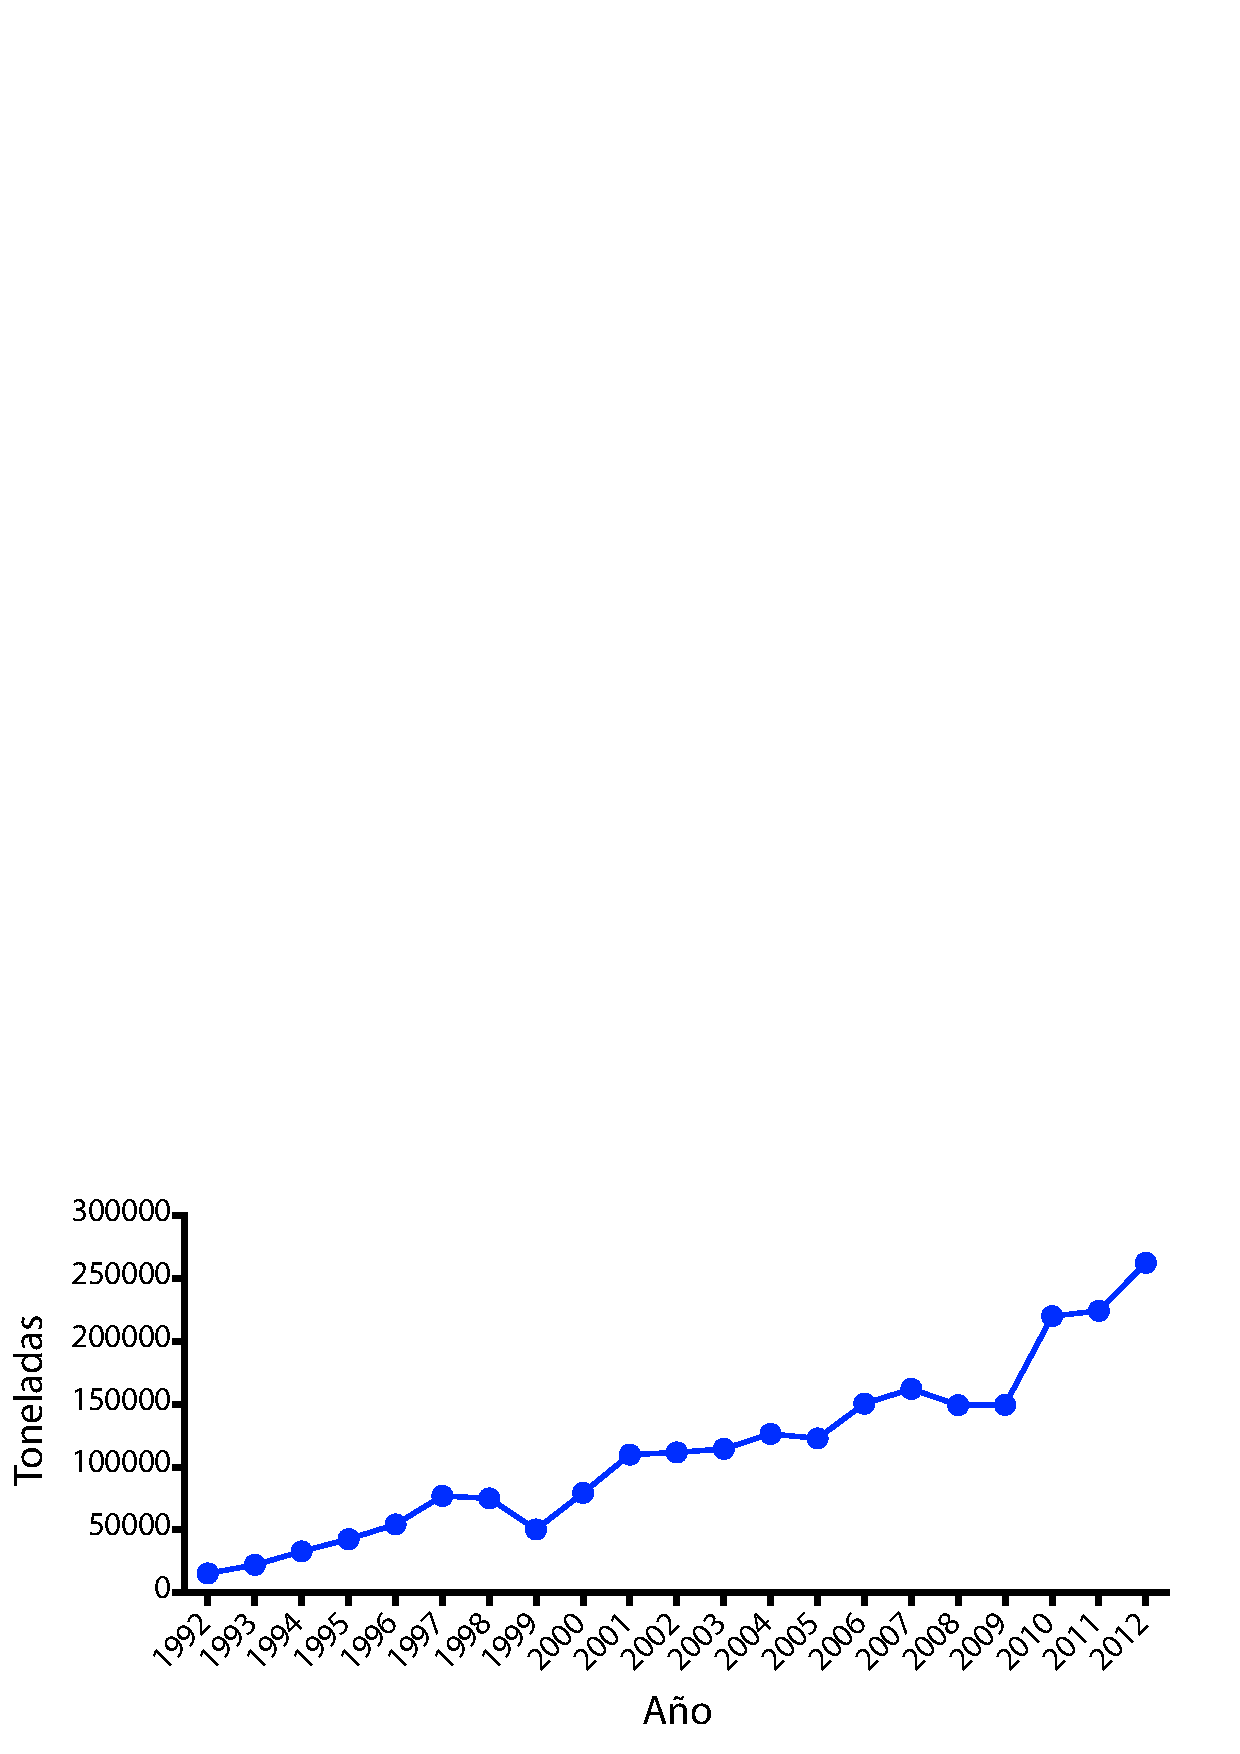
\includegraphics{gfx/desembarques.png}
\caption{Desembarques de Trucha Arcoíris en Chile durante de los ultimos
20 años \label{desembarques}}
\end{figure}

Uno de los principales aspectos a tener en cuenta con una especie con
tal valor comercial es su respuesta inmune. Gran parte de la mortalidad
de estas especies deriva de distintos tipos de infecciones, como por
ejemplo las provocadas por \emph{Flavobacterium psychrophilum} y
\emph{Piscirickettsia salmonis}, llegando a haber muertes en casos de
hasta el 50\% y 34\% de la producción respectivamente. La explicación de
esto radica en la pérdida del equilibrio ambiente-patógeno-hospedero, lo
cual genera las condiciones que hacen aumentar la enfermedad y
mortalidad en el cultivo. En el caso de la acuicultura (Industria que
representa cerca de un 50\% de la oferta mundial de pescado) (FAO,
2012), un grave problema son las enfermedades asociadas a cultivos
masivos de peces, mayoritariamente relacionadas al stress en que se ven
sometidos los organismos como también por el crecimiento acelerado de la
producción y los sistemas de cultivo actuales (FAO, 2012,Georgiadis et
al. (2001))⁠⁠. Estas enfermedades, cualquiera sea su origen, pueden
tener un alto impacto negativo en la producción mundial, lo que equivale
a grandes pérdidas económicas (Shao, 2001)⁠. Por lo tanto es necesario
tener información del sistema inmune en peces, para así poder minimizar
los efectos producidos por estas enfermedades y en algunos casos
prevenirlos.

\subsection{Sistema inmune en peces}\label{sistema-inmune-en-peces}

La comprensión de la funcionalidad del sistema inmune de peces,
especialmente en teleósteos, al igual que en vertebrados superiores se
puede entender como una respuesta innata o inespecífica y una respuesta
adaptativa o especifica. La respuesta inmunológica presentada por los
peces está bien desarrollada e integrada, aunque si, influenciada
notoriamente por los cambios estacionales y la temperatura (Fernández et
al., 2002, Olabuenaga (2000))

La respuesta inmune innata o inespecífica en peces es muy importante, ya
que constituye la primera y más importante línea de defensa del pez
frente a un gran número de patógenos, en esta respuesta convergen
factores humorales y celulares (Fernández et al., 2002). Este tipo de
inmunidad está basado en el reconocimiento no clonal de los componentes
estructurales o secretados de los patógenos microbianos (Athman et al.,
2004)⁠, los cuales son llamados patrones moleculares asociados a
patógenos (o PAMPs, por sus siglas en inglés), estos a su vez son
reconocidos por receptores de reconocimiento de patrón (PRR, por sus
siglas en inglés) (Gordon, 2002), entre los cuales se encuentran
receptores de tipo Toll (TLR, por sus siglas en inglés), el receptor de
complemento tipo-3 (CR3), Dectina-1, proteína C-reactiva, entre otros
(Rondon-Barragan, 2010). Entre los PAMPs más clásicos se puede encontrar
a las secuencias de ADN CpG sin metilar, los lipopolisacáridos (LPS) y
el RNA bicatenario viral. La interacción entre los PRR (como los TLR) y
los PAMP es la reacción que desencadenará e iniciará la transducción de
señales intracelular que resultara en la expresión de genes involucrados
en la inflamación, respuesta antiviral y maduración de células con
fenotipo dendrítico (Aghaallaei et al., 2010)⁠; TLRs individuales
activan factores de transcripción únicos y comunes a través de
diferentes vías de señalización para generar una respuesta biológica
especifica ante microorganismos (Bols et al., 2001)

Entre las células involucradas la fase celular inespecífica de la
respuesta inmune están las células citotóxicas no específicas (NCC, por
sus siglas en inglés), células fagocíticas, y granulocitos (Ainsworth,
1992, Ellis (1977)). Las células NCC en peces se encuentran
principalmente en el riñón cefálico, el bazo, sangre periférica y el
timo, son células citotóxicas inespecíficas, es decir ejercen su acción
en diferentes células diana sin un reconocimiento previo, las cuales
requieren un contacto célula-célula para poder efectuar la lisis celular
(Graves et al., 1984). Dentro de las células fagocíticas los neutrófilos
representan aproximadamente en promedio a un 11\% de los leucocitos en
sangre, son también llamados polimorfonucleares o leucocitos
específicos, su capacidad fagocítica es baja, ya que ingieren poco
material extraño, aunque poseen la mayoría de la batería enzimática para
este trabajo. Los eosinófilos y basófilos son los granulocitos con menor
presencia en peces, aunque en el caso de los eosinófilos se han logrado
encontrar en peritoneo u otros tejidos como el intestino, mientras que
los basófilos tienen escasa presencia en estos organismos (D. Palić et
al., 2011).

Dentro del sistema fagocítico mononuclear, podemos encontrar a los
monocitos y a los macrófagos (derivados de estas últimas), los primeros
son móviles y generalmente más grandes que los demás leucocitos, en el
caso de los macrófagos, pueden fagocitar partículas mucho más grandes,
son abundantes en el bazo y riñón cefálico, aunque también se han
encontrado en mucosa olfatoria (Castro et al., 2011, Olabuenaga (2000)).

Entre los componentes moleculares asociados a la respuesta innata del
sistema inmune de peces podemos encontrar a las citoquinas, las cuales
son una familia de proteínas de bajo peso molecular (comúnmente
glicosiladas) y secretadas por células del sistema inmune activadas
previamente frente a la exposición de diferentes componentes patógenos
(Salazar-Mather et al., 2006)⁠. Estas citoquinas pueden dividirse en
interferones (IFNs), interleuquinas (ILs), factores de necrosis
tumorales (TNFs, por sus siglas en inglés), factores estimuladores de
colonias y quimioquinas (Savan et al., 2006)⁠. Las interleuquinas son
citoquinas producidas principalmente por linfocitos T CD4+, aunque
también son secretadas por una gran variedad de tipos celulares, como
por ejemplo los macrófagos/monocitos y las células endoteliales(C. J.
Secombes et al., 2011), las quimioquinas, o también llamadas citoquinas
quimiotácticas (o quimioatractantes) son una familia de citoquinas que
son liberadas por la mayoría de tejidos infectados en los estadíos
tempranos de infección. Las citoquinas pueden dividirse en distintas
familias según sea la organización de sus cisteínas.

Empezar a hbalar de IL-1B, IFN-g, TNFa iNOS e IL-12

\pagebreak

Otras moléculas efectoras presentes en la respuesta innata frente a
patógenos son los péptidos anti-microbianos (AMP, por sus siglas en
inglés), moléculas con la capacidad de destruir y/o neutralizar
microorganismos patógenos directamente, son moléculas pequeñas,
anfipáticas y catiónicas (Mercado et al., 2005)⁠, y están ampliamente
extendidos por los reinos vegetal y animales (Zasloff, 2002). Los
mecanismos de acción anti-bacteriana de estos AMP pueden entenderse
desde dos puntos de vista diferentes: 1. La estructura anfipática puede
unirse selectivamente a la membrana bacteriana y generar poros
transmembrana, los cuales destruyen a la bacteria desintegrando la
membrana, y 2, los AMP pueden directamente entrar a la bacteria e
interactuar específicamente con factores de crecimiento y metabolismo
bacteriano eventualmente generando la muerte bacteriana (Wimley, 2010,
L.-Y. Zhu et al. (2012))⁠. Entre los péptidos anti microbianos descritos
en peces podemos encontrar cuatro grandes grupos, las defensinas,
proteínas de macrófagos asociadas a resistencia natural (Pramps, por sus
siglas en inglés), NK-lisina y hepcidinas.

Otra familia de péptidos antimicrobianos son las Catelicidinas,
presentes generalmente en neutrófilos y superficies de mucosas, su
actividad se centra principalmente en su interacción con la membrana
plasmática de la bacteria para eventualmente destruirla, fueron
primeramente descritas en mamíferos y luego se han encontrado en
distintos peces teleósteos, algunos casos son los de trucha arcoíris
(C.-i. Chang et al., 2005)⁠, bacalao (Maier et al., 2008), salmón del
atlántico (C.-I. Chang et al., 2006), entre otras.

Además de poseer una robusta y bien desarrollada respuesta inmune innata
como se explicaba anteriormente, los peces también cuentan con una
respuesta adaptativa, con componentes celulares y humorales
(Alvarez-Pellitero, 2008)⁠, en este último grupo se encuentran los
anticuerpos, los cuales son proteínas pertenecientes al grupo de las
inmunoglobulinas (Ig), en el caso de los peces producen inmunoglobulinas
del tipo M, T y D (Bengtén et al., 2002)⁠, siendo la primera la más
importante, estando presente en el suero, el mucus y la bilis. Los
anticuerpos son producidos por linfocitos B activados al reconocer algún
antígeno, ya sea en solución o presentado por alguna célula presentadora
de antígeno, que en el caso de los peces principalmente son macrófagos,
y tienen variadas funciones, pueden actuar como moléculas efectoras en
el suero, o también como receptores de superficie de linfocitos B.

Una de las principales diferencias entre el sistema inmune de peces
teleósteos con el de mamíferos es la carencia de medula ósea y ganglios
linfáticos, por lo cual no se puede marcar una diferencia entre órganos
hematopoyéticos y órganos linfoides (Fernández et al., 2002, Olabuenaga
(2000))⁠. Entre los principales órganos pertenecientes al sistema inmune
de peces podemos encontrar el timo, el riñón y el bazo. El riñón
cefálico es el principal órgano en la diferenciación de linfocitos B, ya
que es el primer órgano en el que aparecen estas células durante el
desarrollo del pez, también es el órgano donde se produce la
eritropoyesis, granulopoyesis, linfopoyesis y monocitopoyesis (Whyte,
2007), por lo que se le puede considerar a la vez un órgano análogo a la
medula ósea de los mamíferos (Razquin et al., 1990)⁠. Los centros
melanomacrofágicos son una agregación de macrófagos que contienen
melanina, un pigmento de color oscuro, su tamaño y número está
directamente relacionado con el estado del pez, ya que estas variables
aumentan considerablemente en peces enfermos, donde el catabolismo ha
sido excesivo. Algunos estudios ontogénicos realizados en salmónidos
sugieren que la función del bazo no es esencial en la maduración del
sistema inmunológico, ya que los linfocitos del timo y riñón cefálico
estarían más involucrados que este órgano en esta maduración. Otros
estudios sin embargo indican, que bajo un desafío antigénico aparecen
linfocitos B en el bazo, teniendo parámetros similares a los presentados
por estas células en otros órganos como el riñón cefálico.

\pagebreak

\subsection{Inmunoestimulantes}\label{inmunoestimulantes}

Los inmunoestimulantes han sido descritos como componentes necesarios
para la acuicultura, ya que mejoran la respuesta innata y proveen
resistencia a patógenos. Diferentes de estas sustancias, como los
B-glucanos, productos bacterianos y constituyentes de las plantas pueden
iniciar directamente la activación de mecanismos de defensa innata
actuando en receptores y desencadenando la activación de distntos genes
que puedan resultar en la producción de moleculas antimicrobianas
(Bricknell et al., 2005, Kumari et al. (2006)). A pesar de la evidencia
demostrada sobre el uso benéfico de estas sustancias como potenciales
inmunomoduladores de la respuesta frente a disntitos patógenos en la
acuicultura (Abarca et al., 2012), las actuales soluciones comerciales
están de cierta manera restringidas por ser derivadas de algunas
levaduras, como por ejemplo los B1-3,B1-6 glucanos que son vendidos bajo
la marca MacroGard® y sus distintos derivados. Existe también un
producto comercial llamado Ergosan, el cual está hecho de una mezcla de
distintos componentes de un alga, la cual es rica en alginatos y
polisacáridos. Una dosis individual de 1mg de Ergosan aumenta
singificativamente la proporción de eutrofilos, aumentan el grado de
fagocitosis, la actividad del estallido respiratorio y la expresión de
interleukina 1B (IL-1B), interleukina 8 (IL-8) y el factor de necrosis
tumoral alfa (TNF-$\alpha$) in leucocitos peritoniales de trucha
arcoíris a 1 dia post inyección (Peddie et al., 2002).

\subsubsection{$\beta$-glucanos}\label{beta-glucanos}

Los $\beta$-glucanos son carbohidratos que consisten en moléculas de
glucosas enlazadas, los cuales son componentes estructurales de gran
importancia en paredes celulares de levaduras, hongos, algas y algunas
bacterias. Estos carbohidratos también forman parte de la pared celular
endospermas de algunos cereales como la cebada y la avena. Dependiendo
del origen del $\beta$-glucano encontraremos diferencias también en sus
estructuras moleculares y sus posibles ramificaciones (Tabla
\ref{tablaglucanos}) (Skov et al., 2012, Volman et al. (2008)).

\begin{table}[h]
\begin{center}
\sffamily
\begin{threeparttable}
\captionsetup{font={normalsize,sf}}
\caption{Estructuras de $\beta$-Glucanos según su origen}\label{tablaglucanos}
\begin{tabular}{l c l}
\toprule
Origen & Estructura & Función \\
\midrule
Bacteriano & \includegraphics[width=0.3\textwidth, height=60mm]{bgbacteriano} & $\beta$1,3-Glucano lineal con ramificaciones largas de $\beta$1,6-Glucano\\
Levadura & \includegraphics[width=0.3\textwidth, height=60mm]{bglevadura} & $\beta$1,3-Glucano Lineal \\ 
Cereal & \includegraphics[width=0.3\textwidth, height=60mm]{bgcereal} & $\beta$1,3/$\beta$1,4-Glucano lineal \\
Hongo & \includegraphics[width=0.3\textwidth, height=60mm]{bghongo} & $\beta$1,3-Glucano lineal con ramificaciones cortas de $\beta$1,6Glucano \\

\bottomrule
\end{tabular}
\begin{tablenotes}
    \item Estructuras de $\beta$-Glucanos según su origen
\end{tablenotes}
\end{threeparttable}
\end{center}
\end{table}

ASDsadsda

\clearpage

\section*{Bibliografía}\label{bibliografuxeda}
\addcontentsline{toc}{section}{Bibliografía}

Abarca, A., Bethke, J., Narváez, E., Flores, R., \& Mercado, L. (2012).
Parameters to evaluate the immunostimulant effect of Zymosan A in head
kidney leucocytes ( HKL ) of salmonids Parámetros para la evaluación del
efecto de Zimosán A como inmunoestimulante sobre leucocitos de riñón
cefálico ( HKL ) de salmónidos, \emph{40}(3), 545--552.

Aghaallaei, N., Bajoghli, B., Schwarz, H., Schorpp, M., \& Boehm, T.
(2010). Characterization of mononuclear phagocytic cells in medaka fish
transgenic for a cxcr3a:gfp reporter. \emph{Proc. Natl. Acad. Sci. U. S.
A.}, \emph{107}(42), 18079--84.

Ainsworth, A. (1992). Fish granulocytes: Morphology, distribution, and
function. \emph{Annu. Rev. Fish Dis.}, \emph{2}, 123--148.

Alvarez-Pellitero, P. (2008). Fish immunity and parasite infections:
from innate immunity to immunoprophylactic prospects. \emph{Vet.
Immunol. Immunopathol.}, \emph{126}(3-4), 171--98.

Athman, R., \& Philpott, D. (2004). Innate immunity via Toll-like
receptors and Nod proteins. \emph{Curr. Opin. Microbiol.}, \emph{7}(1),
25--32.

Bengtén, E., Quiniou, S. M.-A., Stuge, T. B., Katagiri, T., Miller, N.
W., Clem, L. W., \ldots{} Wilson, M. (2002). The IgH Locus of the
Channel Catfish, Ictalurus punctatus, Contains Multiple Constant Region
Gene Sequences: Different Genes Encode Heavy Chains of Membrane and
Secreted IgD. \emph{J. Immunol.}, \emph{169}(5), 2488--2497.

Bilen, S., Bulut, M., \& Bilen, A. M. (2011). Immunostimulant effects of
Cotinus coggyria on rainbow trout (Oncorhynchus mykiss). \emph{Fish
Shellfish Immunol.}, \emph{30}(2), 451--5.

Bols, N. C., Brubacher, J. L., Ganassin, R. C., \& Lee, L. E. (2001).
Ecotoxicology and innate immunity in fish. \emph{Dev. Comp. Immunol.},
\emph{25}(8-9), 853--873.

Bricknell, I., \& Dalmo, R. a. (2005). The use of immunostimulants in
fish larval aquaculture. \emph{Fish Shellfish Immunol.}, \emph{19}(5),
457--72.

Castro, R., Bernard, D., Lefranc, M. P., Six, a, Benmansour, a, \&
Boudinot, P. (2011). T cell diversity and TcR repertoires in teleost
fish. \emph{Fish Shellfish Immunol.}, \emph{31}(5), 644--54.

Chang, C.-i., Pleguezuelos, O., Zhang, Y.-a., Zou, J., \& Secombes, C.
J. (2005). Identification of a novel cathelicidin gene in the rainbow
trout, Oncorhynchus mykiss. \emph{Infect. Immun.}, \emph{73}(8),
5053--64.

Chang, C.-I., Zhang, Y.-A., Zou, J., Nie, P., \& Secombes, C. J. (2006).
Two cathelicidin genes are present in both rainbow trout (Oncorhynchus
mykiss) and atlantic salmon (Salmo salar). \emph{Antimicrob. Agents
Chemother.}, \emph{50}(1), 185--95.

Chettri, J. K., Kania, P. W., \& Buchmann, K. (2013). Immunomodulation
of rainbow trout ( Oncorhynchus mykiss ) fry by bath exposure to a
$\beta$-glucan from Euglena gracilis. \emph{Aquac. Res.}, \emph{44}(9),
1407--1415.

Dalmo, R. a, \& Bøgwald, J. (2008). Beta-glucans as conductors of immune
symphonies. \emph{Fish Shellfish Immunol.}, \emph{25}(4), 384--96.

Ellis, A. E. (1977). The leucocytes of fish: A review. \emph{J. Fish
Biol.}, \emph{11}(5), 453--491.

Ellis, A. E. (2001). Innate host defense mechanisms of fish against
viruses and bacteria. \emph{Dev. Comp. Immunol.}, \emph{25}(8-9),
827--39.

FAO. (2012). \emph{El estado mundial de la pesca y la acuicultura -
2012} (p. 251).

Fernández, A., Ruiz, I., \& Blas, I. D. (2002). El sistema inmune de los
teleósteos (I): Células y órganos. \emph{Rev. Aquat.}, \emph{16}.

Georgiadis, M., Gardner, I., \& Hedrick, R. (2001). The role of
epidemiology in the prevention, diagnosis, and control of infectious
diseases of fish. \emph{Prev. Vet. Med.}, \emph{48}(4), 287--302.

Gordon, S. (2002). Pattern recognition receptors: doubling up for the
innate immune response. \emph{Cell}, \emph{111}(7), 927--30.

Graves, S. S., Evans, D. L., Cobb, D., \& Dawe, D. L. (1984).
Nonspecific cytotoxic cells in fish (Ictalurus punctatus). I. Optimum
requirements for target cell lysis. \emph{Dev. Comp. Immunol.},
\emph{8}(2), 293--302.

Groot, C., \& Margolis, L. (1991). \emph{Pacific Salmon Life Histories}.
University of British Columbia Press.

Kawai, T., \& Akira, S. (2005). Pathogen recognition with Toll-like
receptors. \emph{Curr. Opin. Immunol.}, \emph{17}(4), 338--44.

Kumari, J., \& Sahoo, P. K. (2006). Dietary immunostimulants influence
specific immune response and resistance of healthy and immunocompromised
Asian catfish Clarias batrachus to Aeromonas hydrophila infection.
\emph{Dis. Aquat. Organ.}, \emph{70}(1-2), 63--70.

Maier, V. H., Dorn, K. V., Gudmundsdottir, B. K., \& Gudmundsson, G. H.
(2008). Characterisation of cathelicidin gene family members in
divergent fish species. \emph{Mol. Immunol.}, \emph{45}(14), 3723--30.

Mercado, L., Schmitt, P., Marshall, S. H., \& Arenas, G. (2005). Gill
tissues of the mussel Mytilus edulis chilensis: A new source for
antimicrobial peptides. \emph{Electron. J. Biotechnol.}, \emph{8}(3),
284--290.

Olabuenaga, S. E. (2000). Sistema inmune en peces. \emph{Gayana
(Concepción)}, \emph{64}(2).

Palić, D., Beck, L. S., Palić, J., \& Andreasen, C. B. (2011). Use of
rapid cytochemical staining to characterize fish blood granulocytes in
species of special concern and determine potential for function testing.
\emph{Fish Shellfish Immunol.}, \emph{30}(2), 646--52.

Peddie, S., Zou, J., \& Secombes, C. J. (2002). Immunostimulation in the
rainbow trout (Oncorhynchus mykiss) following intraperitoneal
administration of Ergosan. \emph{Vet. Immunol. Immunopathol.},
\emph{86}(1-2), 101--13.

Razquin, B. E., Castillo, A., Lopez-Fierro, P., Alvarez, F., Zapata, A.,
\& Villena, A. J. (1990). Ontogeny of IgM-producing cells in the
lymphoid organs of rainbow trout, Salmo gairdneri Richardson: an immuno-
and enzyme-histochemical study. \emph{J. Fish Biol.}, \emph{36}(2),
159--173.

Rondon-Barragan, I. (2010). Receptores similares a Toll en peces : el
inicio de la divergencia. \emph{Investig. Vet.}, \emph{11}(1), 15--30.

Salazar-Mather, T., \& Hokeness, K. (2006). Cytokine and Chemokine
Networks: Pathways to Antiviral Defense. In T. E. Lane (ed.),
\emph{Chemokines Viral Infect.} (Vol. 303, pp. 29--46). Springer Berlin
Heidelberg.

Savan, R., \& Sakai, M. (2006). Genomics of fish cytokines. \emph{Comp.
Biochem. Physiol. Part D. Genomics Proteomics}, \emph{1}(1), 89--101.

Secombes, C. J., Wang, T., \& Bird, S. (2011). The interleukins of fish.
\emph{Dev. Comp. Immunol.}, \emph{35}(12), 1336--45.

Sernapesca. (2012). Anuario desembarques. Santiago de Chile: Gobierno de
Chile.

Skov, J., Kania, P. W., Holten-Andersen, L., Fouz, B., \& Buchmann, K.
(2012). Immunomodulatory effects of dietary $\beta$-1,3-glucan from
Euglena gracilis in rainbow trout (Oncorhynchus mykiss) immersion
vaccinated against Yersinia ruckeri. \emph{Fish Shellfish Immunol.},
\emph{33}(1), 111--20.

Subpesca. (2013). Cuenta Pública de Estado de los Recursos. Santiago de
Chile: Gobierno de Chile.

Volman, J. J., Ramakers, J. D., \& Plat, J. (2008). Dietary modulation
of immune function by beta-glucans. \emph{Physiol. Behav.},
\emph{94}(2), 276--84.

Whyte, S. K. (2007). The innate immune response of finfish--a review of
current knowledge. \emph{Fish Shellfish Immunol.}, \emph{23}(6),
1127--51.

Wimley, W. C. (2010). Describing the mechanism of antimicrobial peptide
action with the interfacial activity model. \emph{ACS Chem. Biol.},
\emph{5}(10), 905--17.

Zasloff, M. (2002). Antimicrobial peptides of multicellular organisms.
\emph{Nature}, \emph{415}(6870), 389--95.

Zhang, L., Li, Y.-y., Chen, T., Xia, W., Zhou, Y., Wan, Y.-j., \ldots{}
Xu, S.-q. (2011). Abnormal development of motor neurons in
perfluorooctane sulphonate exposed zebrafish embryos.
\emph{Ecotoxicology}, \emph{20}(4), 643--52.

Zhu, L.-Y., Nie, L., Zhu, G., Xiang, L.-X., \& Shao, J.-Z. (2012).
Advances in research of fish immune-relevant genes: A comparative
overview of innate and adaptive immunity in teleosts. \emph{Dev. Comp.
Immunol.}

\end{document}
